%%%%%%%%%%%%%%%%%%%%%%%%%%%%%%%%%%%%%%%%%
% Journal Article
% LaTeX Template
% Version 1.4 (15/5/16)
%
% This template has been downloaded from:
% http://www.LaTeXTemplates.com
%
% Original author:
% Frits Wenneker (http://www.howtotex.com) with extensive modifications by
% Vel (vel@LaTeXTemplates.com)
%
% License:
% CC BY-NC-SA 3.0 (http://creativecommons.org/licenses/by-nc-sa/3.0/)
%
%%%%%%%%%%%%%%%%%%%%%%%%%%%%%%%%%%%%%%%%%

%----------------------------------------------------------------------------------------
%	PACKAGES AND OTHER DOCUMENT CONFIGURATIONS
%----------------------------------------------------------------------------------------

\documentclass{article}

\NeedsTeXFormat{LaTeX2e}

\usepackage[sc]{mathpazo} % Use the Palatino font
\usepackage[T1]{fontenc} % Use 8-bit encoding that has 256 glyphs
\linespread{1.05} % Line spacing - Palatino needs more space between lines
\usepackage{microtype} % Slightly tweak font spacing for aesthetics

\usepackage[english]{babel} % Language hyphenation and typographical rules

\usepackage[hmarginratio=1:1,top=32mm,columnsep=20pt]{geometry} % Document margins
\usepackage[hang, small,labelfont=bf,up,textfont=it,up]{caption} % Custom captions under/above floats in tables or figures
\usepackage{booktabs} % Horizontal rules in tables

\usepackage{lettrine} % The lettrine is the first enlarged letter at the beginning of the text

\usepackage{enumitem} % Customized lists
\setlist[itemize]{noitemsep} % Make itemize lists more compact

\usepackage{abstract} % Allows abstract customization
\renewcommand{\abstractnamefont}{\normalfont\bfseries} % Set the "Abstract" text to bold
\renewcommand{\abstracttextfont}{\normalfont\small\itshape} % Set the abstract itself to small italic text

\usepackage{titlesec} % Allows customization of titles
\renewcommand\thesection{\Roman{section}} % Roman numerals for the sections
\renewcommand\thesubsection{\roman{subsection}} % roman numerals for subsections
\titleformat{\section}[block]{\large\scshape\centering}{\thesection.}{1em}{} % Change the look of the section titles
\titleformat{\subsection}[block]{\large}{\thesubsection.}{1em}{} % Change the look of the section titles

\usepackage{fancyhdr} % Headers and footers
\pagestyle{fancy} % All pages have headers and footers
\fancyhead{} % Blank out the default header
\fancyfoot{} % Blank out the default footer
\fancyhead[C]{Online community management as social network design} % Custom header text
\fancyfoot[RO,LE]{\thepage} % Custom footer text

\usepackage{titling} % Customizing the title section

\usepackage{hyperref} % For hyperlinks in the PDF

\usepackage{graphicx}
\graphicspath{Pictures/}

\usepackage{subfig}
%----------------------------------------------------------------------------------------
%	TITLE SECTION
%----------------------------------------------------------------------------------------

\setlength{\droptitle}{-4\baselineskip} % Move the title up

\pretitle{\begin{center}\Huge\bfseries} % Article title formatting
\posttitle{\end{center}} % Article title closing formatting
\title{Online community management as social network design: testing for the signature of management activities in online communities} % Article title
\author{\textsc{Alberto Cottica}\thanks{Corresponding author} \\[1ex] \normalsize University of Alicante, Edgeryders \\ \normalsize \href{mailto:alberto@edgeryders.eu}{alberto@edgeryders.eu}\\
\and \textsc{Guy Melançon}\\
[1ex] \normalsize University of Bordeaux \\ 
\and \textsc{Benjamin Renoust} \\[1ex] 
\normalsize National Institute of Informatics \& JFLI CNRS UMI 3527, Tokyo \\ 
}
\date{} % Leave empty to omit a date
\renewcommand{\maketitlehookd}{%
\begin{abstract}
Online communities are used across several fields of human activities, as environments for large-scale collaboration. Most successful ones employ professionals, sometimes called ``community managers'' or ``moderators'', for tasks including onboarding new participants, mediating conflict, and policing unwanted behaviour. Network scientists routinely model interaction across participants in online communities as social networks. We interpret the activity of community managers as (social) network design: they take action oriented at shaping the network of interactions in a way conducive to their community's goals. It follows that, if such action is successful, we should be able to detect its signature in the network itself. 

Growing networks where links are allocated by a preferential attachment mechanism are known to converge to networks displaying a power law degree distribution. Growth and preferential attachment are both reasonable first-approximation assumptions to describe interaction networks in online communities. Our main hypothesis is that managed online communities are characterised by in-degree distributions that deviate from the power law form; such deviation constitutes the signature of successful community management. Our secondary hypothesis is that said deviation happens in a predictable way, once community management practices are accounted for. If true, these hypotheses would give us a simple test for the effectiveness of community management practices. 

We investigate the issue using (1) empirical data on three small online communities and (2) a computer model that simulates a widely used community management activity called \emph{onboarding}. We find that onboarding produces in-degree distributions that systematically deviate from power law behaviour for low-values of the in-degree; we then explore the implications and possible applications of the finding. 
\end{abstract}
}

%----------------------------------------------------------------------------------------

\begin{document}

% Print the title
\maketitle

%----------------------------------------------------------------------------------------
%	ARTICLE CONTENTS
%----------------------------------------------------------------------------------------

\section*{Acknowledgements}
\noindent This paper is based on an earlier version, presented at the Complex Networks 2016 conference \cite{cottica2016testing}

\noindent The authors gratefully acknowledge the invaluable contributions of Giovanni Ponti, Raffaele Miniaci, Noemi Salantiu, Lee-Sean Huang, the faculty and students at University of Alicante and everybody at Masters of Networks 3.

\noindent We acknowledge support of the OPENCARE and CATALYST European projects.

\section{Introduction}

Organizations running online communities typically employ community managers, tasked with encouraging participation and resolving conflict \cite{rheingold1993virtual}. 
These are participants, typically in small numbers (one or two members in the smaller communities) who recognise some central command, and carry out its directives. We shall henceforth call such directives \emph{policies}. 

Putting in place policies for online communities is costly, in terms of community managers recruitment amd training, and software tools. This raises the question of what benefits organisations running online communities expect from policies; and why they choose certain policies, and not others. In what follows we outline and briefly discuss the set of assumptions that underpin our investigation.

\begin{enumerate}
\item We model online communities as social networks of interactions across participants. 
\item We assume that organisations can be modelled as economic agents maximizing some objective function. The target variable being maximised can be profit (for online communities run by commercial companies); or welfare (for online communities run by governments or other nonprofit entities); or some combination of the two. 
\item We assume that the topology of the interaction network characteristic of online communities affects their ability to contribute to the maximisation of the target variable. Indications that this assumption might be reasonable are not difficult to find in the literature \cite{tapscott2008wikinomics},\cite{slegg2014facebook}.
\item We assume that such organisations choose their policies as follows: 
    \begin{itemize} 
	\item Solve their maximisation problem over network topology. This yields a vector of desired network characteristics, where ``desired'' means that those characteristics define a maximum of the objective function. These solutions will be statements with the form ``In order to best meet our ultimate [profit or welfare] goals, the interaction network in our online community should be in state $\Theta_D$'', where $\Theta$ is a vector of topology-related parameters\footnote{The literature on stochastic actor-oriented models goes several steps further, and models interaction in a social network assuming that all participants pursue goals with respect to their position in the network \cite{snijders1996stochastic}. We do not explore this direction in the present paper because such models require the assumption of invariant network size ? or, in our context, a zero-growth online community. We reject such an assumption as too unrealistic.}.
	\item Derive a course of action that community managers could take to change the network away from its present state $\Theta_0$ to the desired state $\Theta_D$.
	\item Encode such course of action in a set of simple instructions for community managers to execute. Computer scientists might think of such instructions as algorithms; economists call them mechanisms; professional online community managers call them policies. In this paper we use this third term. 
    \end{itemize}
\end{enumerate}
All this implies that the decision to deploy a particular policy on an online community is a network design exercise. An organisation decides to employ a community manager to shape the interaction network of its community in a way that helps ist own ultimate goals. 
And yet, interaction networks in online communities cannot really be designed; they are the result of many independent decisions, made by individuals who do not respond to the organization's command structure. An online community management policy is then best understood as an attempt to ``influence'' emergent social dynamics; to use a more synthetic expression, it can be best understood as the attempt to design for emergence. Its paradoxical nature is at the heart of its appeal. 

We are interested in detecting the mathematical signature of specific policies in the network topology. 
We consider a simple policy called \emph{onboarding} \cite{rheingold1993virtual, shirky2008here}. As a new participant becomes active (\emph{e.g.} by posting her first post), community managers are instructed to leave her a comment that contains (a) positive feedback and (b) suggestions to engage with other participants that she might share interests with.

We model online conversations as social networks, and look for the effect of onboarding on the topology of those networks. We proceed as follows:
\begin{enumerate}
\item We initially examine data from three small online communities. Only two of them deploy a policy of onboarding. We observe that, indeed, the shape of the degree distribution of these two differs from that of the third.  
\item We propose an experiment protocol to determine whether onboarding policies can explain the differences observed between the degree distributions of the first two online communities and that of the third one. 
\item Based on a generalized preferential attachment model \cite{dorogovtsev2002evolution}, we simulate the growth of online communities. Variants to the model cover the relevant cases: the absence of onboarding policies and their presence, with varying degrees of effectiveness. 
\item We run the experiment protocol against the degree distributions generated by the computer model, and discuss its results.
\end{enumerate}
Section 2 briefly examines the two strands of literature that we mostly draw upon. Section 3 presents some data from real-world online communities; it then proceeds to describe our main experiment, a computer simulation of interaction in online communities with and without onboarding. Section 4 presents the experiment's results. Section 5 discusses them.
%------------------------------------------------

\section{Related works}

The extraordinary successes of online communities in deploying large-scale, decentralized projects has led many scholars to conjecture that online communities exhibit emergent behavior, and called such behavior collective intelligence, after an influential book by Pierre L\'evy \cite{pierre1997collective}. This name was adopted by a research community that aims at providing tools for better collective sense- and decision making such as argument maps (representations of the logical structure of a debate, with all redundancy eliminated) \cite{shum2003roots} and attention-mediation metrics (indicators that signal what, in an online debate, is worthiest reading and responding to. The number of Likes on Facebook is one such metric) \cite{klein2012enabling}. 

Collective intelligence scholars confirmed importance of online community management practices, indeed, they have tried to systematize it \cite{diplaris2011emerging} and produce technological innovation to support it \cite{shum2003roots, de2012contested}. 
These tools are meant to facilitate and encourage participation to online communities, to make it easier for individuals to extract knowledge from them.
Studying human communities is a traditional focus of network science \cite{borgatti2009network, burt2009structural}, for which  easily available datasets of online communities make an ideal ground for structural analysis: friendship in Facebook \cite{lewis2008tastes, nick2013toward}, following/retweet/mentions for Twitter \cite{kunegis2013preferential, java2007we, hodas2014simple}, or vote and comments in discussions \cite{hodas2014simple, laniado2011wikipedians, zhang2007expertise, zanetti2012quantitative}. 

Starting in the 2000s, online communities became the object of another line of enquiry, stemming from network science. Network representation of relationships across groups of humans has yielded considerable insights in social sciences since the work of the sociometrists in the 1930s, and continues to do so; phenomena like effective spread of information, innovation adoption, and brokerage have all been addressed in a network perspective \cite{borgatti2009network, burt2009structural}. As new datasets encoding human interaction became available, many online communities came to be represented as social networks. This was the case for social networking sites, like Facebook \cite{lewis2008tastes, nick2013toward}; microblogging platform like Twitter \cite{kunegis2013preferential, java2007we, hodas2014simple}; news-sharing services like Digg \cite{hodas2014simple}; collaborative editing projects like Wikipedia \cite{laniado2011wikipedians}; discussion forums like the Java forum \cite{zhang2007expertise}; and bug reporting services for software developers like Bugzilla \cite{zanetti2012quantitative}. Generally, such networks represent participants as nodes. Edges represent a relationship or interaction. The nature of interaction varies across online communities: one edge can stand for friendship for Facebook; follower-followed relationship, retweet or mention in Twitter; vote or comment in Digg and the Java forum; talk in Wikipedia; comment in Bugzilla. 

In contrast to collective intelligence scholars, network scientists typically do not address the issue of community management, and treat social networks drawn from online interaction as fully emergent. In this paper, we employ a network approach to investigate the issue of whether the work of community managers leaves a footprint detectable by quantitative analysis. To our knowledge, no other work attempted this investigation.
In particular, we exploit a result from the theory of evolving networks, from seminal work by Barab\'asi and Albert \cite{barabasi1999emergence} showing that the assumption of growth and preferential attachment, when taken together, result in a network whose degree distribution converges to a power law ( \cite{barabasi2005origin, barabasi1999mean}). The model was later generalized in various ways and tested across a broad range of networks, including social networks 
\cite{dorogovtsev2002evolution}. 

We use this generalized model as a baseline. The degree distribution of the interaction network in an online community follows a power law by default. The action of online community managers, as they attempt to further the goals of the organisation that runs the online community, will result in its degree distribution deviating from the baseline power law in predictable ways. Such deviation can be interpreted as the signature that the policy is working well. 

The most important difficulty with this method is the absence of a counterfactual: if a policy is enacted in the online community, the baseline degree distribution corresponding to the absence of the policy is not observable, and viceversa. This rules out a direct proof that the policy ``works''. Hence our choice to combine empirical data and computer simulations. 

%------------------------------------------------

\section{Materials and methods}
\label{sec:materials}
In this section we introduce the empirical data, the experiment protocol and the simulation model we use in the experiment. 

\subsection{Empirical data}
\label{sec:empirical_data}

We examine data from three real-world online communities. All three use the same software (Drupal 7), are roughly comparable in size and are used by practitioners and interested citizens to publicly discuss issues that have a collective dimension. They are modelled as interaction networks, in which nodes are registered users and edges represent comments. The presence of an edge from Alice to Bob indicates that Alice has commented content authored by Bob at least once. The resulting graphs are directed (``Alice comments Bob'' is not equivalent to ``Bob comments Alice'') and weighted (Alice can write multiple comments to Bob's content; the edge's weight is equal to the number of comments written). Table \ref{table:empiricalData} presents some descriptive statistics about them. 

\begin{itemize}
\item InnovatoriPA is a community of (mostly) Italian civil servants discussing how to introduce and foster innovation in the public sector. It does not employ any special onboarding or moderation policy. 
\item Edgeryders is a community of (mostly) European citizens, discussing public policy issues from the perspective of grassroot activism and social innovation. It enacts the onboarding of new members policy. 
\item Matera 2019 is a community of (mostly) citizens of the Italian city of Matera and the surrounding region, discussing the city's policies.
It, too, enacts an onboarding policy.
\end{itemize}

% careful here. The numbers in the table refer to the in-degree distributions, not to the **transformed** in-degree distributions. Also (and for this reason) the lower bound is constrained to k >= 1 rather than k > 1.
\begin{table*}[t]
\centering 
\begin{tabular}{| c | c | c | c |} 
\hline 
& \textbf{Innovatori PA} & \textbf{Edgeryders} & \textbf{Matera2019}\\ 
\hline
Policy & \emph{``no special policy''} & \emph{``onboard new users''} & \emph{``onboard new users''}\\ 
\hline 
In existence since & December 2008 & October 2011 & March 2013 \\
Accounts created & 10,815 & 2,419 & 512 \\
\hline 
Active participants (nodes) & 619 & 596 & 198 \\
Number of edges (weighted) & 1,241 & 4,073 & 883 \\
\hline 
Average distance & 3.77 & 2.34 & 2.51 \\
Maximum degree & 155 & 238 & 46 \\
Average degree & 2.033 & 6.798 & 4.454 \\
\hline 
\multicolumn{4}{c} {\textbf{Goodness-of-fit for $k \geq 1$}}\\
\hline
exponent & 1.611 & 1.477 & 1.606 \\
$p$-value & 0.21 & 0.00 (reject) & 0.00 (reject)\\
\hline
\multicolumn{4}{c} {\textbf{Goodness-of-fit for $k \geq k_{min}$}}\\
\hline
$k_{min}$ & 2 & 5 & 6 \\
exponent & 1.834 & 2.250 & 2.817 \\
$p$-value & 0.76 & 0.45 & 0.94 \\
\hline
\end{tabular}
\caption{Comparing interaction networks of the three online communities and testing for goodness-of-fit of power functions to degree distributions. ``Exponent'' refers to the power law's scaling parameter. ``$p$-value'' to the result of the test that the degree distribution of the community was generated by a power law with that exponent. \vspace{-0 cm}}
\label{table:empiricalData}
\end{table*}

The communities are modeled as interaction networks (summarized in Table \ref{table:empiricalData}) in which nodes are users and edges represent directed comments from $A$ to $B$, weighted by the number of comments written. A glance at their respective visualizations (Figure\,\ref{fig:NetViz}) suggests that the networks of the three communities have very different topologies. Innovatori PA displays more obviously visible hubs than the other two. 

\begin{figure}[t]
\centering
	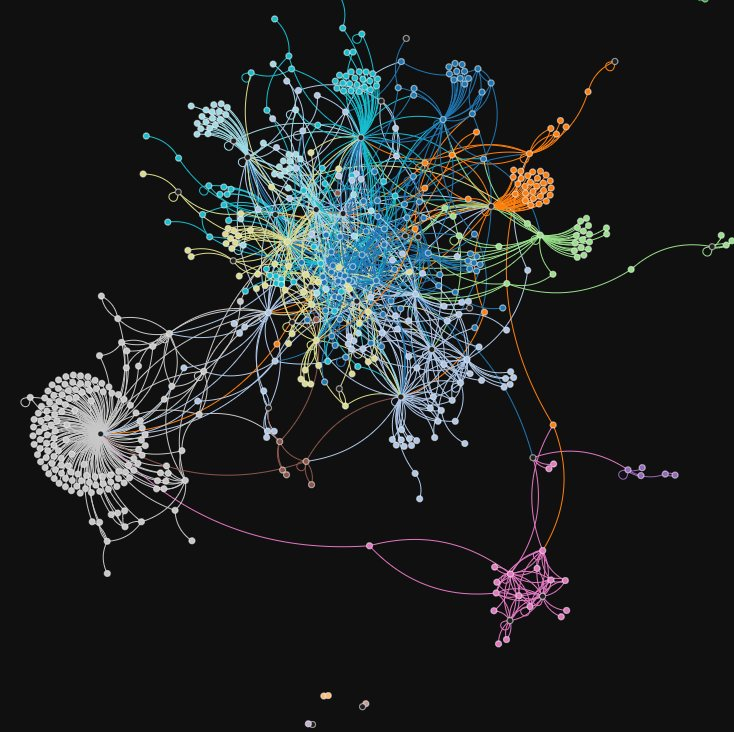
\includegraphics[width=.32\linewidth]{./Pictures/innovatoripa_01}\label{fig:InnoNet}
	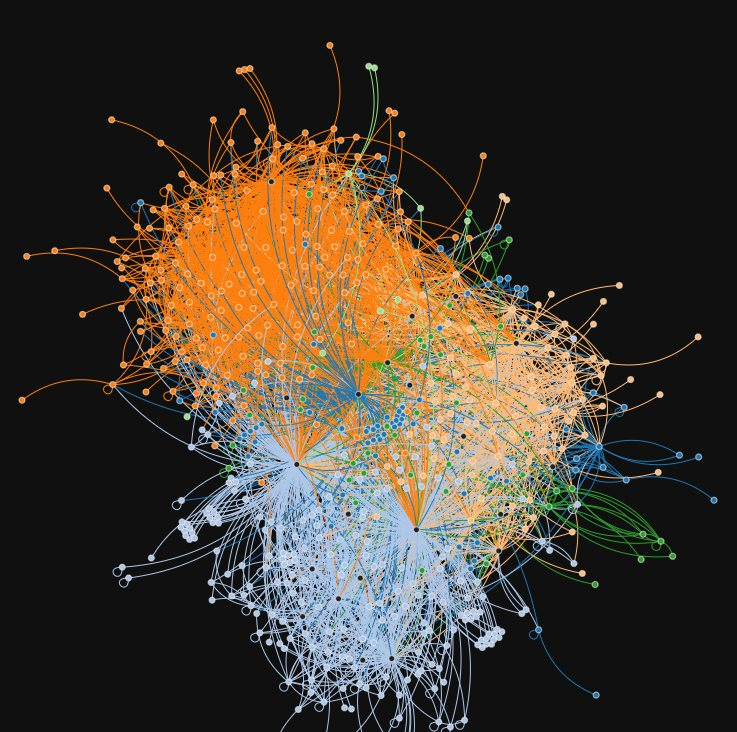
\includegraphics[width=.32\linewidth]{./Pictures/edgeryders_02}\label{fig:EdgeNet}
  	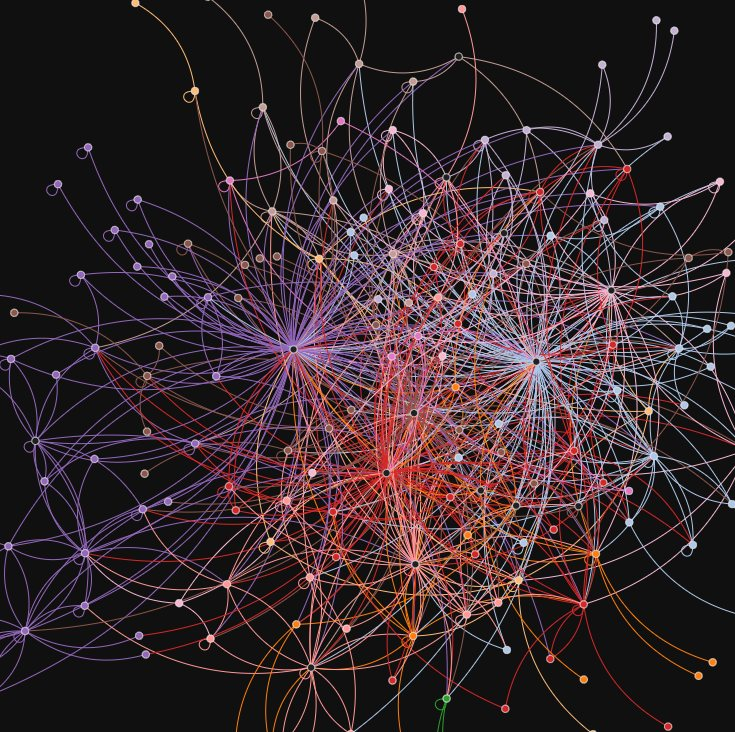
\includegraphics[width=.32\linewidth]{./Pictures/matera2019_01}\label{fig:MT2019Net}
  \caption{Interaction networks of three small online communities. Innovatori PA (left) does not have an onboarding policy in place, whereas the two others do (Edgeryders: center, Matera: right). \vspace{-.5cm}} 
 \label{fig:NetViz}
\end{figure}

We fitted power laws in-degree distributions of these three online communities, as of early December 2014. Next, we tested the hypothesis that degree distributions follow a power law, as predicted by \cite{dorogovtsev2002evolution}. To do so, we first fitted power functions to the entire support of each in-degree distribution\footnote{We emphasize in-degree, as opposed to out-degree, 
because directedness is implicit in the idea of preferential attachment, and because the in-degree distribution is the one to follow a power law in online conversation networks \cite{dorogovtsev2002evolution}.
}. We next fitted power functions to the right tail of each in-degree distribution, \emph{i.e.} for any degree $k(n) \geq k_{min}$, where $q_{min}$ is the in-degree that minimizes the Kolmogorov-Smirnov distance (hereafter denoted as $D$) between the fitted function and the data with in-degree $k \geq k_{min}$. 

% the above: same thing. k should be constrained to k > 1

Finally, we ran goodness-of-fit (hereafter $GoF$) tests for each in-degree distribution and for fitted power functions. The method we followed throughout the paper is borrowed from Clauset \emph{et al} \cite{clauset2009power}. The null hypothesis tested is that the observed distribution is generated by a power function with exponent $\alpha$. We compare the $D$ statistic of the observed distribution with those of a large number of synthetic datasets drawn by the fitted power function. Such comparison is summarised in a $p$-value, that indicates the probability of the $D$ statistic to exceed the observed value conditional to the null hypothesis being true. $p$-values close to 1 indicate that the power function is a good fit for the data: the null hypothesis is not rejected. $p$-values close to zero indicate that the power function is a bad fit for the data, and reject the null hypothesis. The rejection value is set, conservatively, at 0.1. Results are summarised in Table \ref{table:empiricalData}. 
	
% this figure: power law is fitted to in-degree distribution, not transformed IDD
	
\begin{figure*}
\makebox[\textwidth]{
\subfloat[fig:_flow_example][]{
	\includegraphics[width=.5\linewidth]{./Pictures/PDF_innovatoriPA}\label{fig:fit_innovatoriPA}
}
\subfloat[fig:_fit_no_onboarding][]{
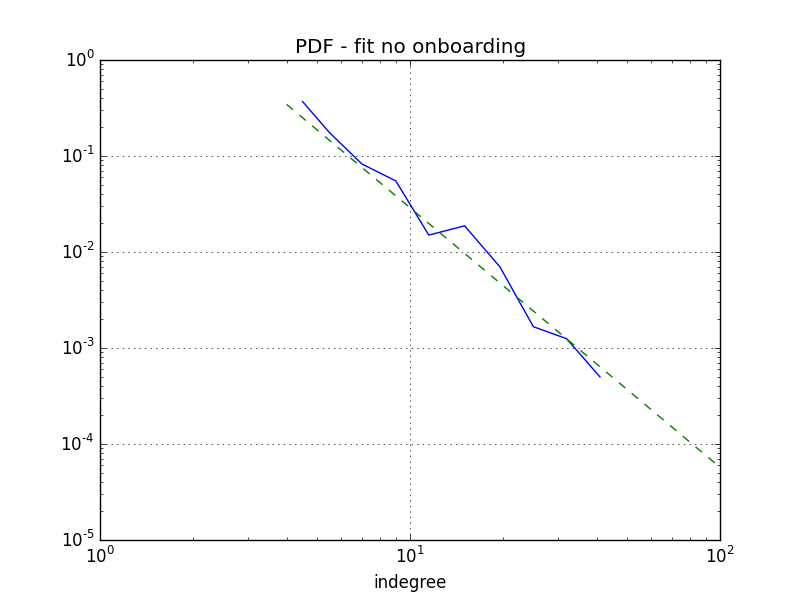
\includegraphics[width=.5\linewidth]{./Pictures/PDF_fit_no_onboarding_0049}\label{fig:fit_no_onboarding}
}
}
\\
\makebox[\textwidth]{
\subfloat[fig:_fit_edgeryders][]{
	\includegraphics[width=.5\linewidth]{./Pictures/PDF_edgeryders}\label{fig:fit_edgeryders}
}
\subfloat[fig:_fit_nu_1_1][]{
	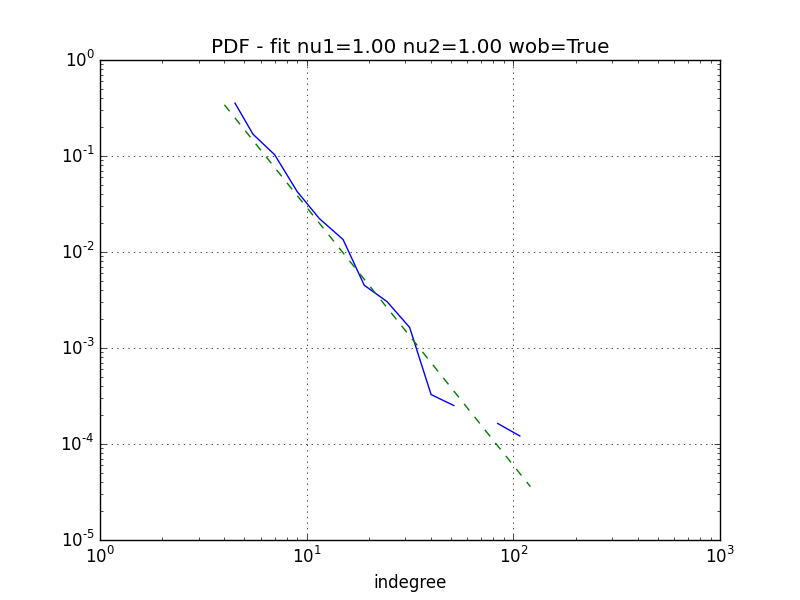
\includegraphics[width=.5\linewidth]{./Pictures/PDF_fit_nu1_1_nu2_1_wob_True_0049}\label{fig:fit_nu_1_1}
}
}
\caption{($\log$ - $\log$) Probability density function from the transformed degree distributions of: (a) the Innovatori PA network without onboarding policy in place versus (b) a simulated network with preferential attachment and no onboarding.
(c) The Edgeryders network with onboarding and preferential attachment versus (d) a simulated network with preferential attachment and fully effective onboarding ($\nu_1 = \nu_2 = 1$).\vspace{-.5cm}}
 \label{fig:PDFViz}
\end{figure*}


As we consider the interval  $q \geq 1$, we find that the in-degree distribution of the Innovatori PA network -- the unmoderated one -- is consistent with the expected behavior of an evolving network with preferential attachment. We cannot reject the null hypothesis that it was generated by a power law. For other two communities, both with onboarding policies, the null hypothesis is strongly rejected. On the other hand, when we consider only the tail of the degree distributions, i.e. $k \geq k_{min}$, all three communities display a behavior that is consistent of a setting with preferential attachment.

These results are consistent with the objectives of the onboarding policy, consisting in helping newcomers find their way around a community that they don't know yet. A successfully onboarded new user will generally have some extra interaction with existing active members. All things being equal, we can expect extra edges to appear in the network, and interfere with the in-degree distribution that would appear in the absence of onboarding -- explaining the non-power law distribution of Edgeryders and Matera2019. Extra edges target mostly low connectivity nodes: onboarding targets newcomers, and focuses on helping them through the first few successful interactions. Highly active (therefore highly connected) members do not need to be onboarded. This may explain why all three communities display power law behavior in the upper tail of their in-degree distributions, regardless of onboarding. 

\subsection{Experiment protocol}
\label{ss:experiment_protocol}
The difference observed between the two communities with onboarding policies and the one without might be caused not by the policy itself, but by some other unobserved variable. To explore the issue further, we generate and compare computer simulations of interaction networks in online communities that are identical except for the presence and effectiveness of onboarding policies. Communities are assumed to grow over time, with new participants joining them in sequence; at each point in time, new edges appear; their probability of targeting an existing node grows linearly with that node's in-degree. Additionally, communities might have or not have onboarding policies. For those communities that do have them, they are modelled by means of two scalar parameters $\nu_1$  and $\nu_2$ , that vary between 0 and 1. The first one captures onboarding effectiveness;  the second one captures community responsiveness. As they get closer to 1, the community manager's onboarding action gets closer to having the desired effects. In the next subsection, we specify the model and define more specifically the meaning of both parameters.

We proceed as follows.

First, we simulate the evolution of the interaction network of a large number of online communities. Divide them into a control group (no onboarding policy) and a treatment group (presence of onboarding policy). Specifically, we simulate the evolution of the interaction network of:

\begin{itemize}
\item 100 communities with no onboarding policy. These will constitute the control group of our simulated communities. 
\item 100 communities for each couple of values of $\nu_1$  and $\nu_2$, with $\nu_1, \nu_2 \in \{0.0, 0.2, 0.4, 0.6, 0.8, 1.0\}$. These will constitute our treatment groups.
\item For each of these networks, we compute the in-degree distribution.
\end{itemize}

Next, we define the following hypotheses. 


\begin{itemize}
\item Let $C$ be the network of interaction in an online community. Denote the in-degree of nodes in the network by $k$. Let $F$ be the best-fit power-law model for the distribution 

\begin{equation}
\label{eq:tIDD}
 q(k) = k + mA
\end{equation}
 
 where $k$ is the in-degree distribution of $C$, $m$ the number of nodes that join the network at each timestep and $A$ a node attractiveness parameter.
\item \emph{Hypothesis 1}. The distribution of $q(k)$ is generated by $F$ for any $k > 1$\footnote{The exact formulation in \cite{dorogovtsev2002evolution} is $k > > 1$. We simplify it to $k > 1$, because onboarding only targets newcomers to an online community, therefore low-degree nodes in the network. That is where we expect the goodness-of-fit of the transformed in-degree distribution to the power law model to break down. We are therefore especially interested in looking at the lower tail of the distribution.}.
\item \emph{Hypothesis 2}. The distribution $q(k)$ is generated by $F$ for any $k \geq k_{min}$, where $k_{min}$ is the in-degree that minimizes the Kolmogorov-Smirnov distance between the fitted function and the data over $k \geq k_{min}$.
\end{itemize}

Both hypotheses are based on the asymptotic form taken by the stationary in-degree distribution of networks growing by preferential attachments in \cite{dorogovtsev2002evolution}. The result holds even if preferential attachment is not the sole mode of network evolution, and for any edge sources.

Finally, we test Hypothesis 1 and 2 on each of the 3700 in-degree distributions generated. We do this using the goodness-of-fit tests proposed by Clauset et.al. \cite{clauset2009power} and illustrated in detail in the Appendix. We expect to obtain the following:

\begin{itemize}
\item In the control group, both Hypothesis 1 and Hypothesis 2 are true. 
\item In the treatment group with fully effective onboarding Hypothesis 1 is false and Hypothesis 2 is true. 
\item In the intermediate situations of partially ineffective onboarding, Hypothesis 1 can be true or false, according to the value of $\nu_1$ and $\nu_2$. Hypothesis 2 is true.
\end{itemize}


%-------------------------------------------------

\section{Results}\label{sec:results}
Following the protocol outlined above, we evolved 100 networks for each of the 37 variants of the model. For all networks, we set network size to 2000 nodes; $A = 1$; and $m = 1$. These choices are discussed in the Appendix.

\subsection{Goodness-of-fit of the power-law model} \label{ssec:GOF of power law}

For each network evolved we computed two best-fit power-law models, one for $k > 1$ and the other for $k\geq k_{min}$ where $k_{min}$ is the in-degree the minimizes the Kolmogorov-Smirnov distance between the fitted function and the data over $k \geq k_{min}$. On each of these models, we ran a goodness-of-fit test as described in Section \ref{ss:experiment_protocol}. This resulted in two distributions of $p$-values for our control group, plus two more for each of our six treatment groups. Table \ref{table:GOF1}
 and \ref{table:AvgPvc} report descriptive statistics for these distributions.

\begin{table}[h] 
\centering
\caption{Number of rejects (out of 100 runs) for goodness-of-fit tests of power-law models to in-degree distributions of interaction networks in online communities, with no onboarding (control group) and with onboarding. Power-law models are estimated over all nodes with degree $k > 1$}
\label{table:GOF1}
\begin{tabular}{lcccccc}
\hline
\multicolumn{7}{c} {Control group: 61}\\
\hline
\quad & \quad $\nu_2$ = 0.0 \quad & \quad $\nu_2$ = 0.2 \quad & \quad $\nu_2$ = 0.4 \quad & \quad $\nu_2$ = 0.6 \quad & \quad $\nu_2$ = 0.8 \quad & \quad $\nu_2$ = 1\quad \\
\quad $\nu_1$ = 0.0          \quad & \quad 99        \quad & \quad 97        \quad & \quad 100        \quad & \quad 99        \quad & \quad 99        \quad & \quad 100      \quad \\
\quad $\nu_1$ = 0.2          \quad & \quad 100        \quad & \quad 100        \quad & \quad 99        \quad & \quad 98        \quad & \quad 97        \quad & \quad 98      \quad \\
\quad $\nu_1$ = 0.4          \quad & \quad 98        \quad & \quad 98        \quad & \quad 96        \quad & \quad 99        \quad & \quad 100        \quad & \quad 98      \quad \\
\quad $\nu_1$ = 0.6          \quad & \quad 96        \quad & \quad 96        \quad & \quad 99        \quad & \quad 99        \quad & \quad 99        \quad & \quad 98      \quad \\
\quad $\nu_1$ = 0.8          \quad & \quad 98        \quad & \quad 97        \quad & \quad 98        \quad & \quad 99        \quad & \quad 98        \quad & \quad 98      \quad \\
\quad $\nu_1$ = 1            \quad & \quad 98        \quad & \quad 98        \quad & \quad 100        \quad & \quad 100        \quad & \quad 99        \quad & \quad 98   \quad \\
\hline  
\end{tabular}
\end{table}

From Table \ref{table:GOF1}, we conclude that onboarding seems to have some effect on the goodness-of-fit of the generated data to their respective best-fit power-law models when $k > 1$. The effect goes in the direction of reducing the $p$-values and increasing the number of rejects to almost 100\%.  

It is worth looking at the average $p$-values generated by each combination of $\nu_1$ and $\nu_2$. These are shown in Table \ref{table:AvgPvc}.

\begin{table}[h]
\centering
\caption{Average $p$-values for goodness-of-fit tests of power-law models to in-degree distributions of interaction networks in online communities, with no onboarding (control group) and with onboarding. Power-law models are estimated over all nodes with degree $k > 1$}
\label{table:AvgPvc}
\begin{tabular}{lllllll}
\hline
\multicolumn{7}{c} {Control group: 0.183}\\
\hline
Average $p$-value \quad & \quad $\nu_2$ = 0.0 \quad & \quad $\nu_2$ = 0.2 \quad & \quad $\nu_2$ = 0.4 \quad & \quad $\nu_2$ = 0.6 \quad & \quad $\nu_2$ = 0.8 \quad & \quad $\nu_2$ = 1  \quad \\
\quad $\nu_1$ = 0.0       \quad & \quad 0.005  \quad & \quad 0.010  \quad & \quad 0.005   \quad & \quad 0.007  \quad & \quad 0.006  \quad & \quad 0.007 \quad \\
\quad $\nu_1$ = 0.2       \quad & \quad 0.005  \quad & \quad 0.006  \quad & \quad 0.009  \quad & \quad 0.011  \quad & \quad 0.014  \quad & \quad 0.012 \quad \\
\quad $\nu_1$ = 0.4       \quad & \quad 0.009  \quad & \quad 0.009     \quad & \quad 0.015  \quad & \quad 0.005  \quad & \quad 0.006  \quad & \quad 0.008  \quad \\
\quad $\nu_1$ = 0.6       \quad & \quad 0.013    \quad & \quad 0.012  \quad & \quad 0.008   \quad & \quad 0.009  \quad & \quad 0.010  \quad & \quad 0.008 \quad \\
\quad $\nu_1$ = 0.8       \quad & \quad 0.009  \quad & \quad 0.015  \quad & \quad 0.012  \quad & \quad 0.009  \quad & \quad 0.012  \quad & \quad 0.009 \quad \\
\quad $\nu_1$ = 1         \quad & \quad 0.009  \quad & \quad 0.011  \quad & \quad 0.009  \quad & \quad 0.008  \quad & \quad 0.010  \quad & \quad 0.013\quad \\
\hline
\end{tabular}
\end{table} 

We run $t$-tests of the null hypothesis that the average $p$-value in the control group is equal to the average $p$-values in each ofthe different treatment groups. This results in a strong rejection of the null for any combination of $\nu_1$ and $\nu_2$ ($6.5 < T < 7.5$ in all cases). It seems unquestionable that introducing onboarding to an online community has a measurable negative impact on the probability of a power-law model to be a good fit for its interaction network's in-degree distribution.

We now turn to the question of the role played by $\nu_1$ and $\nu_2$ within the treatment group. Figure \ref{fig:CDFpvcnu_1nu_2} show the cumulate density functions of the $p$-values in the control and treatment groups as $\nu_1$ and $\nu_2$ vary. 

\begin{figure}[thb]
\centering

	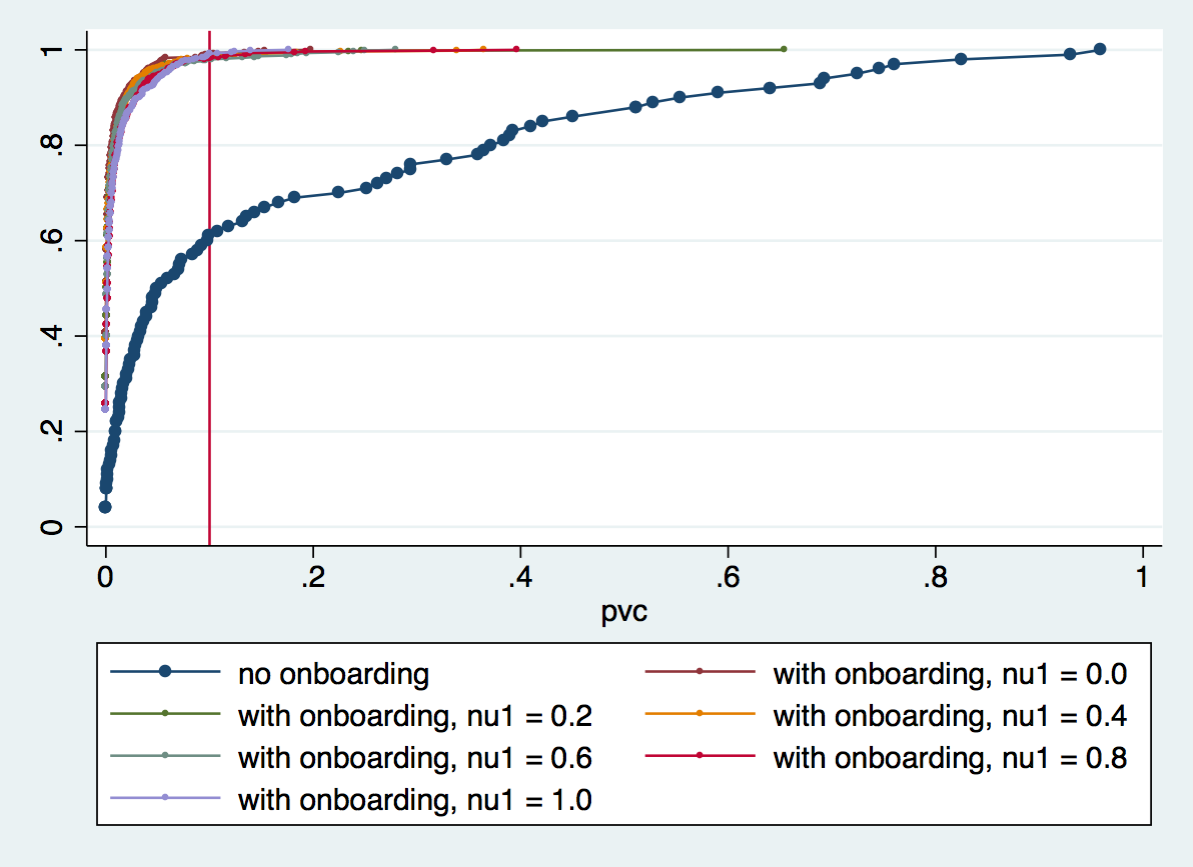
\includegraphics[width=.75\linewidth]{./Pictures/CDF_pvc_nu1.png}\label{fig:CDFnu_1}
	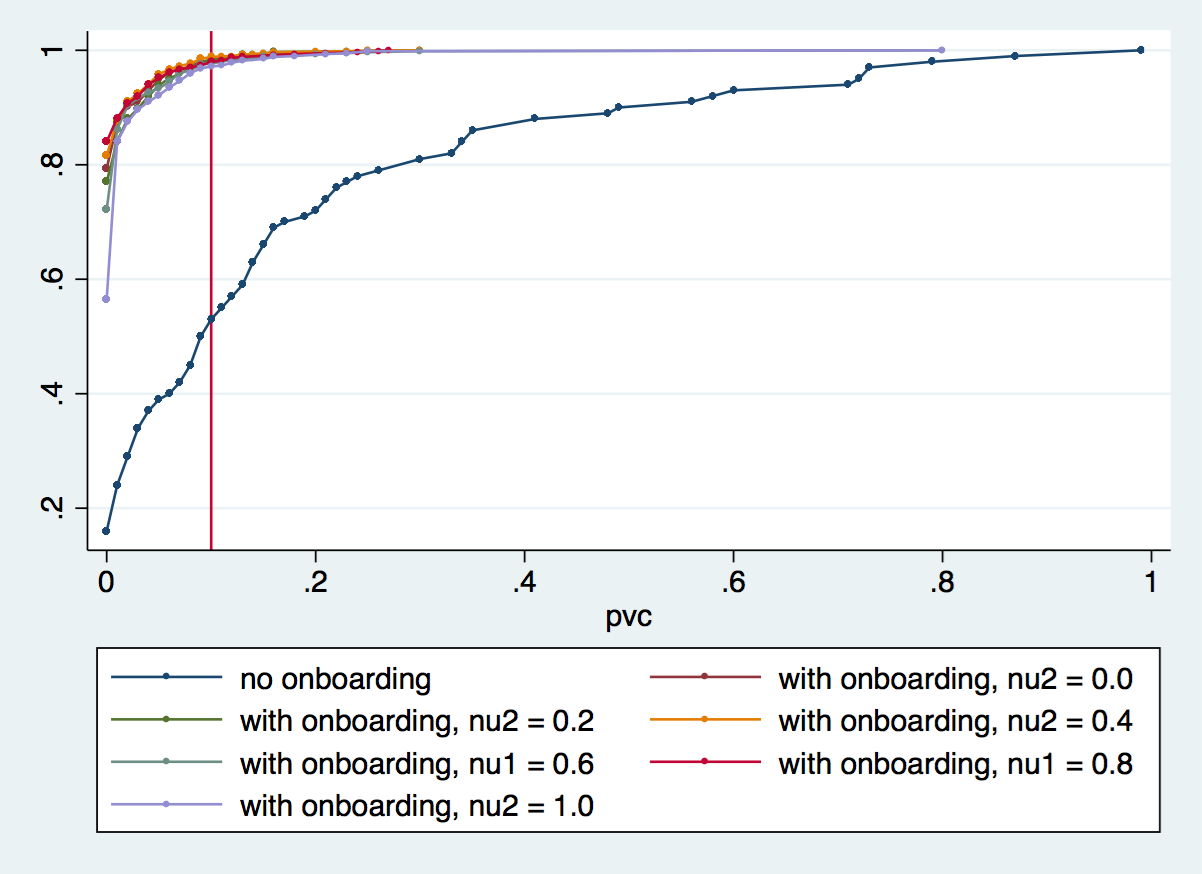
\includegraphics[width=.75\linewidth]{./Pictures/CDF_pvc_nu2.png}\label{fig:CDFnu_2}
  %\subfloat[][]{}
  %\subfloat[][]{}
  \caption{Cumulate Density Functions of $p$-values returned by goodness-of-fit tests to the (best-fit) power-law models for in-degree distributions of the interaction networks in the control and treatment groups. 60\% of the networks evolved without onboarding (dark blue) have degree distributions that test negatively for H1. When onboarding is introduced, that percentage rises to almost 100\%. Above, the treatment group interaction networks have been grouped according to the value taken by $\nu_1$; below, they have been grouped according to the value taken by $\nu_2$ } 
 \label{fig:CDFpvcnu_1nu_2}
\end{figure}

Onboarding effectiveness $\nu_1$ and community responsiveness $\nu_2$ do not seem seem to affect the goodness-of-fit to power law of in-degree distributions much. This is likely to be simply an effect of the large impact of onboarding: the percentage of non-power law distributions is already close to 100\% and cannot increase any further.

Regression analysis confirms the intuition from Figure \ref{fig:CDFpvcnu_1nu_2}. We generated 6 dummy variables, each taking value 1 when $\nu_1 =  c$ and 0 otherwise, with $c \in \{0.0, 0.2, 0.4, 0.6, 0.8, 1\}$; next we generated 6 more dummy variables for the same vaules of $\nu_2$ . We then estimated a linear regression model with the $p$-value of our goodness-of-fit test (computed for $k >1$) as the dependent variable and the 12 dummy variables as its predictors. The results are:

\begin{enumerate}
\item Coefficients on predictors corresponding to different values of $\nu_1$ are positive, but generally non-significant. The coefficient on the variable corresponding to $\nu_1 = 0.4$ is weakly significant ($p$-value: 0.026).
\item Coefficients on predictors corresponding to different values of $\nu_2$ are also  positive and non-significant. 
\item Coefficients on several interaction terms between $\nu_1$ and $\nu_2$ are not significant. 
\item We ran $F$-tests of joint significance of the group of predictors corresponding to different values of $\nu_1$; different values of $\nu_2$; and the interaction terms thereof. The null hypothesis of non-significance was not rejected by any of the tests. 
\end{enumerate}

Similar results hold when $p$-values are computed for $k > k_{min}$. 

When we consider only the upper tail of the the distribution generated by equation \ref{eq:tIDD}, the effect of introducing onboarding on the goodness-of-fit is much less clear. In Table \ref{table:rejectsUnconstrained} we show what happens when we choose the scaling range so as to minimize the Kolmogorov-Smirnov distance between the degree distributions themselves and their best-fit power-law models. In the control group, the goodness-of-fit-to-power-law test fails in 13 of the 100 runs. In the treatment groups, rejections vary from 18 to 36, depending on the values of $\nu_1$ and $\nu_2$.  

\begin{table}[h]
\centering
\caption{Number of rejects (out of 100 runs) for goodness-of-fit tests of power-law models to in-degree distributions of interaction networks in online communities, with no onboarding (control group) and with onboarding. Power-law models are estimated over all observations with $k \geq k_{min}$}
\label{table:rejectsUnconstrained}
\begin{tabular}{lllllll}
\hline
\multicolumn{7}{c} {Control group: 13}\\
\hline
 \quad & \quad $\nu_2$ = 0.0 \quad & \quad $\nu_2$ = 0.2 \quad & \quad $\nu_2$ = 0.4 \quad & \quad $\nu_2$ = 0.6 \quad & \quad $\nu_2$ = 0.8 \quad & \quad $\nu_2$ = 1\quad \\
\quad $\nu_1$ = 0.0        \quad & \quad 34        \quad & \quad 35        \quad & \quad 35        \quad & \quad 25        \quad & \quad 22        \quad & \quad 28      \quad \\
\quad $\nu_1$ = 0.2          \quad & \quad 35        \quad & \quad 24        \quad & \quad 30        \quad & \quad 34        \quad & \quad 29        \quad & \quad 29      \quad \\
\quad $\nu_1$ = 0.4          \quad & \quad 28        \quad & \quad 22        \quad & \quad 25        \quad & \quad 34        \quad & \quad 27        \quad & \quad 26      \quad \\
\quad $\nu_1$ = 0.6          \quad & \quad 29        \quad & \quad 27        \quad & \quad 18        \quad & \quad 23        \quad & \quad 28        \quad & \quad 19      \quad \\
\quad $\nu_1$ = 0.8          \quad & \quad 26        \quad & \quad 27        \quad & \quad 28        \quad & \quad 36        \quad & \quad 32        \quad & \quad 18      \quad \\
\quad $\nu_1$ = 1            \quad & \quad 28        \quad & \quad 28        \quad & \quad 18        \quad & \quad 27        \quad & \quad 21        \quad & \quad 27   \quad \\
\hline  
\end{tabular}
\end{table}

Average $p$-values of goodness-of-fit tests when $k \geq k_{min}$ are shown in Table \ref{table:AvgPvu}. They are all well within the do-not-reject range. The control group has an average $p$-value which is \textit{lower} than that of the treatment group, which is somehow counterintuitive. 

Tables \ref{table:rejectsUnconstrained} and \ref{table:AvgPvu} tell two different stories. Table \ref{table:rejectsUnconstrained} is unconclusive: in both the control and the treatment groups, we do not reject Hypothesis 2 in the treatment group most of the time, as expected, but must still reject in a relatively large number of cases (13 in the control group, 18-36 in the treatment groups). Table \ref{table:AvgPvu} indicates that the average $p$-value in all groups is comfortably within the do-not-reject range, and in this sense behaves entirely according to Hypothesis 2. 

\begin{table}[h]
\centering
\caption{Average $p$-values for goodness-of-fit tests of power-law models to in-degree distributions of interaction networks in online communities, with no onboarding (control group) and with onboarding. Power-law models are estimated over all observations with $k \geq k_{min}$}
\label{table:AvgPvu}
\begin{tabular}{lllllll}
\hline
\multicolumn{7}{c} {Control group: 0.451}\\
\hline
Average $p$-value \quad & \quad $\nu_2$ = 0.0 \quad & \quad $\nu_2$ = 0.2 \quad & \quad $\nu_2$ = 0.4 \quad & \quad $\nu_2$ = 0.6 \quad & \quad $\nu_2$ = 0.8 \quad & \quad $\nu_2$ = 1  \quad \\
\quad $\nu_1$ = 0.0       \quad & \quad 0.341  \quad & \quad 0.341  \quad & \quad 0.345   \quad & \quad 0.368  \quad & \quad 0.411  \quad & \quad 0.355 \quad \\
\quad $\nu_1$ = 0.2       \quad & \quad 0.328  \quad & \quad 0.399  \quad & \quad 0.364  \quad & \quad 0.339  \quad & \quad 0.324  \quad & \quad 0.381 \quad \\
\quad $\nu_1$ = 0.4       \quad & \quad 0.382  \quad & \quad 0.408     \quad & \quad 0.367  \quad & \quad 0.341  \quad & \quad 0.414  \quad & \quad 0.372  \quad \\
\quad $\nu_1$ = 0.6       \quad & \quad 0.348    \quad & \quad 0.372  \quad & \quad 0.4087   \quad & \quad 0.381  \quad & \quad 0.413  \quad & \quad 0.409 \quad \\
\quad $\nu_1$ = 0.8       \quad & \quad 0.370  \quad & \quad 0.383  \quad & \quad 0.382  \quad & \quad 0.324  \quad & \quad 0.359  \quad & \quad 0.436 \quad \\
\quad $\nu_1$ = 1         \quad & \quad 0.383  \quad & \quad 0.401  \quad & \quad 0.458  \quad & \quad 0.413  \quad & \quad 0.4  \quad & \quad 0.393\quad \\
\hline
\end{tabular}
\end{table}  

\subsection{Lower bounds} \label {ssec:lower bounds}

Our results show a limited, albeit statistically significant, effect of onboarding on the value of $k_{min}$, the value of $k$ that minimizes the Kolmogorov-Smirnov distance between the data generated by the computer simulation and the best-fit power-law model. Table \ref {table:ttestkMin} illustrates, for each value of  $\nu_1$ and $\nu_2$, the average value of $k_{min}$, and the result (expressed in $p$-value) of a $t$-test on the null hypothesis that such average value is the same as the corresponding statistics in the control group, against the alternative hypothesis that the former is greater than the latter. 


% Heads up!  xmin in the powerlaw package refers to qmin in the sense of equation (1), not to k_min. Since q = k + ma = k + 1, a value of xmin of 3 is equivalent to a k_min of 2. I manually rescaled all the xmins in the table below.

\begin{table}[h]
\centering
\caption{Average values of $k_{min}$ in the control group and in the treatment group by values of $\nu_1$ and $\nu_2$. The number in parenthesis is the $p$-value associated to a $t$-test that  $k_{min}(treatment) = k_{min}(control)$. }
\label{table:ttestkMin}
\begin{tabular}{lllllll}
\hline
\multicolumn{7}{c} {Control group: 1.87}\\
\hline
  \quad & \quad $\nu_2$ = 0.0 \quad & \quad $\nu_2$ = 0.2 \quad & \quad $\nu_2$ = 0.4 \quad & \quad $\nu_2$ = 0.6 \quad & \quad $\nu_2$ = 0.8 \quad & \quad $\nu_2$ = 1\quad \\
\quad $\nu_1$ = 0.0        \quad & \quad 2.23 (0.006)        \quad & \quad 2.3 (0.003)         \quad & \quad 2.38 (0.001)        \quad & \quad 2.33 (0.001)        \quad & \quad 2.48 (0.000)        \quad & \quad 2.34 (0.001)      \quad \\
\quad $\nu_1$ = 0.2          \quad & \quad 2.42 (0.000)        \quad & \quad 2.45 (0.000)        \quad & \quad 2.46 (0.000)        \quad & \quad 2.36 (0.001)        \quad & \quad 2.33 (0.001)        \quad & \quad 3.3 (0.004)      \quad \\
\quad $\nu_1$ = 0.4          \quad & \quad 2.51 (0.000)        \quad & \quad 2.68 (0.000)        \quad & \quad 2.44 (0.000)        \quad & \quad 2.27 (0.007)        \quad & \quad 2.49 (0.000)        \quad & \quad 2.59 (0.000)      \quad \\
\quad $\nu_1$ = 0.6          \quad & \quad 2.42 (0.000)        \quad & \quad 2.35 (0.001)        \quad & \quad 2.63 (0.000)        \quad & \quad 2.5 (0.000)        \quad & \quad 2.53 (0.000)        \quad & \quad 2.65 (0.000)      \quad \\
\quad $\nu_1$ = 0.8          \quad & \quad 2.44 (0.000)        \quad & \quad 2.54 (0.000)        \quad & \quad 2.49 (0.000)        \quad & \quad 2.34 (0.001)        \quad & \quad 2.26 (0.007)        \quad & \quad 2.56 (0.000)      \quad \\
\quad $\nu_1$ = 1            \quad & \quad 2.55 (0.000)         \quad & \quad 2.52 (0.000)        \quad & \quad 2.66 (0.000)        \quad & \quad 2.58 (0.000)        \quad & \quad 2.5 (0.000)        \quad & \quad 2.49 (0.000)   \quad \\
\hline  
\end{tabular}
\end{table}

% Heads up! The pictures are also generated taking the transformation into account. kmin = x_min - 1

\begin{figure}[thb]
\centering

	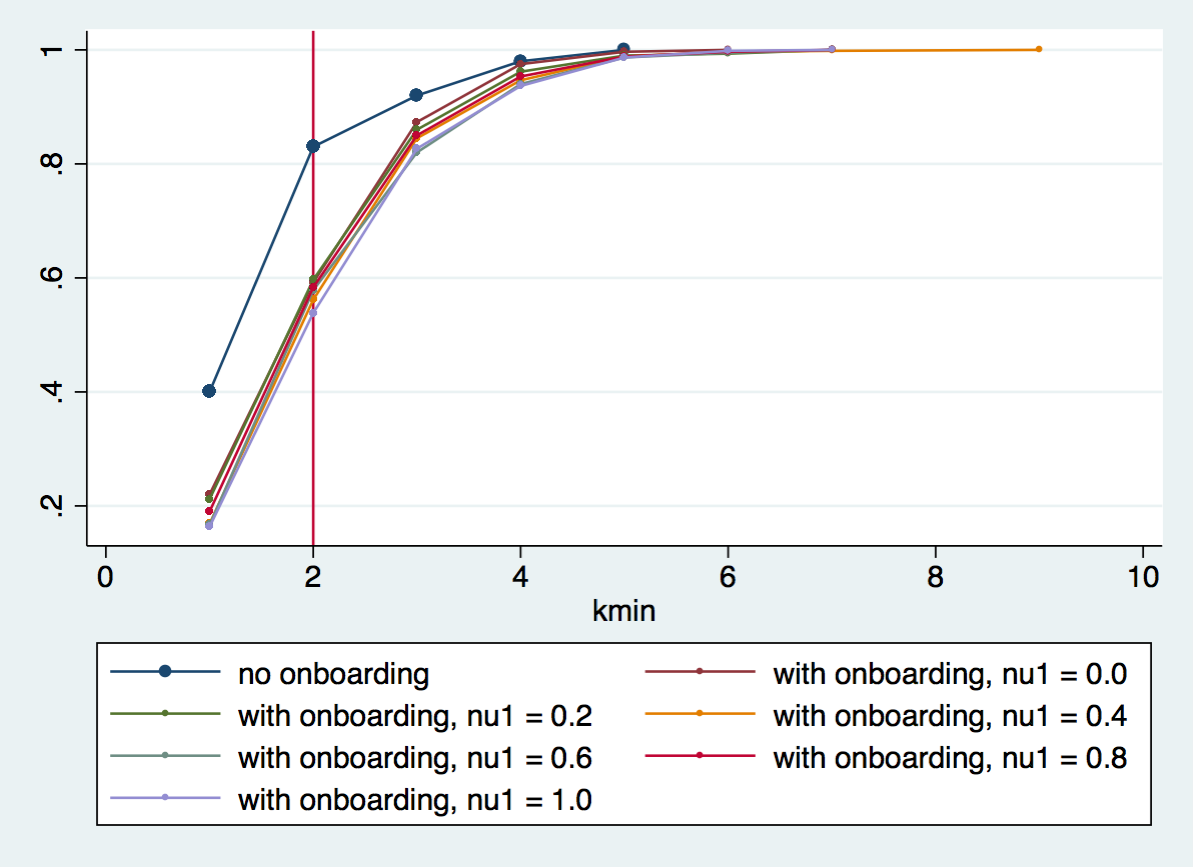
\includegraphics[width=.75\linewidth]{./Pictures/CDF_kmin_nu1.png}
	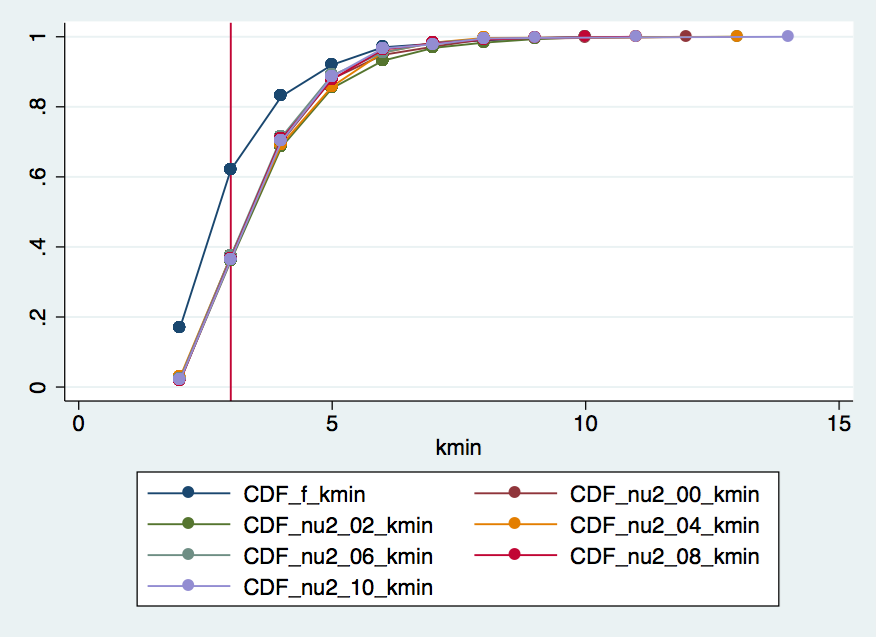
\includegraphics[width=.75\linewidth]{./Pictures/CDF_kmin_nu2.png}
  %\subfloat[][]{}
  %\subfloat[][]{}
  \caption{Cumulate Density Functions of the average value of $k_{min}$ that minimizes the Kolmogorov-Smirnov distance between the in-degree distribution of each interaction network and its best-fit power-law model in the control and treatment groups. 20\% of the networks evolved without onboarding (dark blue) have degree distributions that test negatively for H1. When onboarding is introduced, that percentage rises to between 50 and 90\%. Above, the treatment group interaction networks have been grouped according to the value taken by $\nu_1$; below, they have been grouped according to the value taken by $\nu_2$.} 
 \label{fig:CDFkmin_nu_1nu_2}
\end{figure}

A glance at Figure \ref{fig:CDFkmin_nu_1nu_2} shows that over 80\% of the in-degree distributions from interaction networks in the control group, vis-a-vis only 50 to 60\% of those in the treatment group, fit a power-law model best for $k_{min} \leq 2$. Within the treatment group, no significant variability seems to be associated to the increase of either $\nu_1$ or $\nu_2$. Regression analysis confirms this.

\subsection{Exponents} \label{ssec:exponents}
We find that introducing onboarding to an online community has a positive and significant effect on the value of the exponent of the best-fit power-law model for the in-degree distribution of its interaction network, as computed on $k > 1$. This is consistent with the theoretical results by Dorogovtsev and Mendes \cite{dorogovtsev2002evolution}, who proved that introducing a fraction of non-preferential attachment edges in evolving networks with preferential attachment does not suppress the power-law dependence of its degree distribution, but only increases the scaling exponent thereof. 

This result holds when the best-fit power-law models is computed over $k \geq k_{min}$, where $k_{min}$ is, as usual, the value of $k$ that minimizes the Kolmogorov-Smirnov distance between the simulated in-degree distribution and its best-fit power-law model. When it is computed over the whole support of the in-degree distribution ($k \geq  1$), it also holds, except for $\nu_1 = 1$; in this case, the null hypothesis that the values of the exponents in the control and in the treatment groups are not statistically distinguishable. Tables \ref {table:ttestExpA} and \ref {table:ttestExp} illustrate, for each value of  $\nu_1$ and $\nu_2$, the average value of the scaling parameter $\alpha$, and the result (expressed in $p$-value) of a $t$-test on the null hypothesis that such average value is the same as the corresponding statistics in the control group, against the alternative hypothesis that the former is greater than the latter. Table \ref{table:ttestExpA} refers to $k \geq  1$, whereas Table \ref{table:ttestExp} refers to $k_{min}$.

\begin{table}[h]
\centering
\caption{Average values of the power-law model's exponent $\alpha$ in the control group and in the treatment group by values of $\nu_1$ and $\nu_2$, computed over $k > 1$. The number in parenthesis is the $p$-value associated to a $t$-test that  $\alpha(treatment) = \alpha(control)$. We only show $p$-values greater it the difference is non-significant at the 0.01 level. }
\label{table:ttestExpA}
\begin{tabular}{lllllll}
\hline
\multicolumn{7}{c} {Control group: 2.52}\\
\hline
  \quad & \quad $\nu_1$ = 0.0 \quad & \quad $\nu_2$ = 0.2 \quad & \quad $\nu_2$ = 0.4 \quad & \quad $\nu_2$ = 0.6 \quad & \quad $\nu_2$ = 0.8 \quad & \quad $\nu_2$ = 1\quad \\
\quad $\nu_1$ = 0.0        \quad & \quad 3.03         \quad & \quad 3.03          \quad & \quad 3.03        \quad & \quad 3.03         \quad & \quad 3.03         \quad & \quad 3.03      \quad \\
\quad $\nu_1$ = 0.2          \quad & \quad 2.87         \quad & \quad 2.87        \quad & \quad 2.88        \quad & \quad 2.87         \quad & \quad 2.87         \quad & \quad 2.87       \quad \\
\quad $\nu_1$ = 0.4          \quad & \quad 2.76         \quad & \quad 2.76         \quad & \quad 2.76      \quad & \quad 2.76       \quad & \quad 2.76        \quad & \quad 2.76       \quad \\
\quad $\nu_1$ = 0.6          \quad & \quad 2.67        \quad & \quad 2.67        \quad & \quad 2.67      \quad & \quad  2.67         \quad & \quad 2.66        \quad & \quad 2.66      \quad \\
\quad $\nu_1$ = 0.8          \quad & \quad 2.59         \quad & \quad 2.59         \quad & \quad 2.59        \quad & \quad 2.59        \quad & \quad 2.59        \quad & \quad 2.59      \quad \\
\quad $\nu_1$ = 1            \quad & \quad 2.53 (0.08)         \quad & \quad 2.53 (0.05)        \quad & \quad 2.53 (0.03)        \quad & \quad 2.53 (0.10)        \quad & \quad 2.53 (0.01)        \quad & \quad 2.53 (0.04)   \quad \\
\hline  
\end{tabular}
\end{table}

\begin{table}[h]
\centering
\caption{Average values of the power-law model's exponent $\alpha$ in the control group and in the treatment group by values of $\nu_1$ and $\nu_2$, computed over$k \geq k_{min}$. We omit the $p$-values associated to a $t$-test that  $\alpha_{treatment} = \alpha_{control}$, as they are smaller than 0.01 in all cases. }
\label{table:ttestExp}
\begin{tabular}{lllllll}
\hline
\multicolumn{7}{c} {Control group: 2.64}\\
\hline
 \quad & \quad $\nu_2$ = 0.0 \quad & \quad $\nu_2$ = 0.2 \quad & \quad $\nu_2$ = 0.4 \quad & \quad $\nu_2$ = 0.6 \quad & \quad $\nu_2$ = 0.8 \quad & \quad $\nu_2$ = 1\quad \\
\quad $\nu_1$ = 0.0        \quad & \quad 3.29        \quad & \quad 3.30        \quad & \quad 3.30    \quad & \quad 3.30    \quad & \quad 3.32        \quad & \quad 3.30       \quad \\
\quad $\nu_1$ = 0.2          \quad & \quad 3.12        \quad & \quad 3.13        \quad & \quad 3.13        \quad & \quad 3.11        \quad & \quad 3.11        \quad & \quad 3.09      \quad \\
\quad $\nu_1$ = 0.4          \quad & \quad 2.97        \quad & \quad 2.99        \quad & \quad 2.97        \quad & \quad 2.95        \quad & \quad 2.97        \quad & \quad 2.98      \quad \\
\quad $\nu_1$ = 0.6          \quad & \quad 2.85        \quad & \quad 2.84        \quad & \quad 2.87        \quad & \quad 2.86        \quad & \quad 2.86        \quad & \quad 2.87      \quad \\
\quad $\nu_1$ = 0.8          \quad & \quad 2.76        \quad & \quad 2.77        \quad & \quad 2.77        \quad & \quad 2.75    \quad & \quad 2.74        \quad & \quad 2.77      \quad \\
\quad $\nu_1$ = 1            \quad & \quad 2.69       \quad & \quad 2.69        \quad & \quad 2.70        \quad & \quad 2.70        \quad & \quad 2.69        \quad & \quad 2.68   \quad \\
\hline  
\end{tabular}
\end{table}

We inspect further the impact of parameters $\nu_1$ and $\nu_2$ via regression analysis. It shows that the former has a significant impact, whereas the latter does not. To prove this, we proceed analogously to Section \ref{ssec:GOF of power law}: we estimate two linear regression models with the 12 dummy variables as its predictors. In the first one, the dependent variable is the value of the power-law model's exponent $\alpha$ when the model is estimated over $k > 1$ for each interaction network. In the second one, the dependent variable is power-law model's exponent $\alpha$ when the model is estimated over $k \geq k_{min}$. The results for both models are very similar.

\begin{enumerate}
\item Coefficients on predictors corresponding to different values of $\nu_1$ are negative and highly significant, though small.
\item Coefficients on predictors corresponding to different values of $\nu_2$ are non-significant.
\item Coefficients on interaction terms between $\nu_1$ and $\nu_2$ are non-significant.
\item A $F$-test of joint significance of the group of predictors corresponding to different values of $\nu_1$ strongly rejects the null hypothesis of non-significance. 
\item A $F$-test of joint significance of the group of predictors corresponding to different values of $\nu_2$ does not reject the null hypothesis of non-significance.
\item A $F$-test of joint significance of the interaction terms does not reject the null hypothesis of non-significance.
\end{enumerate}.

\section{Discussion}

\subsection{Accounting for degree distribution shape in the interaction networks of online communities}

Our simulation model incorporates two forces. The first one is preferential attachment; the second is onboarding. The former is meant to represent the rich-get-richer effect observed in many real-world social networks; the latter is meant to represent the onboarding action of moderators and community managers. The former's effect is known to lead to the emergence of an in-degree distribution that approximates a power-law model. The latter's effect is more subtle, because it is in turn composed of two effects. The first one consists in the direct action of the moderator, which  always targets the newcomer; the second one in the actions that might be undertaken as a result of well-executed onboarding policy. 

The direct action of the moderators creates edges pointing to nodes not selected by preferential attachment. What (non-moderator) participants in the online community do as a result of moderator activity is not as clear-cut. In our simulation model, successful onboarding ($\nu_1, \nu_2 > 0$) results in extra edges, some of which point to nodes selected by preferential attachment, others to nodes selected otherwise. 

Also, onboarding always targets newcomers to online communities. It is concerned with weakly connected participants in the community: moderators have no need to engage with very active, strongly connected participants, who clearly need no help in getting a conversation going. By doing so, moderators hope to help shy newcomers turn into active community members. Once this process is under way moderators have no reason to continue to engage with the same individuals. In terms of our model, this means that newcomers, after having being onboarded, are going to receive new edges by preferential attachment only. It is therefore reasonable to expect that the degree distributions generated by our model display a heavy tail, with the frequency of highly connected nodes following a reasonable approximation of a power law. At the same time, power law behaviour is ``drowned out'' by non-preferential attachment edges being created at low levels of $k$. This is indeed what we observe. The overall result of onboarding, then, is an in-degree distribution with power-law behavior for high values of in-degree $k$ and non-power law behavior for low (close to 1) values of $k$. 

Onboarding policies lead to a poorer fit of power-law models to the in-degree distributions of the interaction networks of online communities. This effect shows in the three key parameters that describe power law models. When onboarding is enacted:

\begin {enumerate}
\item $p$-values of the bets-fit power low models are lower. 
\item The values of $k$ that minimise the Kolmogorov-Smirnov distance between the best-fit power-law models and the observed data are greater. 
\item Scaling parameters are greater: onboarding makes the allocation of incoming edges more equal. 
\end{enumerate}

Our specification of the model accounts for an apparent paradox: the deviation of the observed networks' degree distributions from power-law behaviour is \emph{greater} when onboarding is ineffective than when it is effective. This is clearest as we examine the effect of increasing Table \ref{table:ttestExpA}. When onboarding is fully effective ($\nu_1 = 1$), the difference between the average exponent with respect to the control group disappears. Ineffective onboarding only adds edges directly created by moderators, none of which are allocated across existing nodes by preferential attachment. As onboarding gets more effective, even more edges are added; some are allocated by preferential attachment, and drive the degree distribution back towards a more pure power-law behavior. 

The community responsiveness parameter in our model does not appear to impact the shape of the in-degree distribution. This is somewhat surprising: using the control group as a benchmark, executing the onboarding policy adds, at each time step, one edge whose target is not allocated by preferential attachment, and this one edge seems to have a significant impact in pulling the shape of the in-degree distribution away from a good fit with a power-law model for weakly connected nodes. Yet, when we add a second non-preferential attachment allocated edge (via community response to the newcomer reaching out), this does not appear to have any additional impact\footnote{This statement concerns only the shape of the in-degree distribution, the focus of this paper. Other characteristics of the interaction networks are naturally influenced by community responsiveness; higher values of the responsiveness parameter leads to a greater number of edges, and therefore, all other things being equal, to higher connectivity, lower average distance and so on. }.

\subsection{Limitations}

We undertook this research work in the hope of discovering a simple empirical test that could be used to assess the presence and effectiveness of online community management policies, onboarding among them. The guiding idea is that the agency of online community managers and moderators is guided by a logic \textit{other} than the rich-get-richer dynamics that spontaneously arises in many social networks. Such dynamics is associated to power-law shaped degree distributions, which we can regard as the default state for social interaction networks: we conjecture that, whenever the interaction network of an online community does not have the shape of a power law, some agency is at work. We furthermore conjecture that the precise nature of such deviations can be interpreted, and ultimately that different social forces at work on an online community each leave their different mathematical signatures on the community's interaction network. Such signatures could, in principle, be read in the precise form of the deviation of the degree distribution from its default state. 

Our results are in accordance with the first of the two conjectures. Applying onboarding to our simulated community, in whatever form, results in degree distributions that are markedly more distant from pure power-law behaviour than we find in our control group. However, we do not find a monotonic relationship between onboarding's effectiveness and the distance of the resulting degree distribution from a pure power-law form. Hence, when we observe real-world online communities whose interaction networks do not have a full power-law form (like those of Section \ref{sec:empirical_data}), we cannot conclude that it is successfully onboarding its members as they join. At best, we could confirm that their community managers are at work. But we could not assess how successful they are, solely on the basis of the in-degree distribution of the communities' interaction networks\footnote{Furthermore, we could obviously not tell the signature of onboarding to those of other online community management policies. Not, at least, without further study. In fairness, the use case we have in mind for our empirical test is of an organisation who has instructed its community manager to onboard new members as they join, and wishes to assess the quality of their work.}. 

Even simple detection of onboarding is problematic. In this study, we simulate a large  number of online communities, both with and without onboarding, and get our results by comparing the groups with each other. In the real world, however, a researcher might be interested in detecting onboarding in one single online community. Here, our results are inconclusive. If a power law model is a good fit for the in-degree distribution of the community's interaction network (transformed as per equation \ref{eq:tIDD}), an onboarding policy is unlikely to be present. This is because almost all communities with onboarding fail the goodness-of-fit test (table \ref{table:GOF1}). But the reverse does not hold. If we applied the test to our real-world online community and rejected the hypothesis that it was generated by a power law model, it would be difficult to draw any conclusion. This is, of course, because many communities without onboarding fail the goodness-of-fit test as well. 

\subsection{Directions for future research}

There are three obvious directions in which our work could be taken further. The first is a full and systematic exploration of the parameter space, with the goal of assessing our results' robustness with respect to model specification. In this paper we restrict ourselves to the presence and effectiveness of the onboarding action in a baseline model which is closely modeled on Dorogovtsev's and Mendes's results \cite{dorogovtsev2002evolution}; it would be useful to test for how these results carry through as we alter other parameters of the model, such as the number of edges $m$ created at each time step, and the additional attractiveness parameter $A$. 

A second direction for further research is to attempt to make the model into a more realistic description of a real-world online community. Such an attempt would draw attention onto how some real-world phenomena, when incorporated in the model, influence its results. It would also carry the advantage of allowing online community management professional to more easily interact with the model and critique it. Several issues that could be investigated in this vein come to mind. For example, we could relax the assumption that the additional attractiveness parameter $A_s$ is identical for all nodes, allowing for different nodes in the network to attract incoming edges at different rates (a phenomenon known as multiscaling \cite{bianconi2001competition}). Secondly, we could introduce a relationship between out-degree and in-degree: this would reflect the fact that, in an online community, reaching out to others (which translates in increasing one's own out-degree in the interaction network) is a good way to get noticed and attract incoming comments (which translates in increasing one's in-degree)\footnote{This would mean taking an approach conceptually (but not mathematically) similar to stochastic actor-oriented modelling \cite{snijders1996stochastic}.}. Thirdly, we could work with online community manager professionals to model more precisely the action of online community managers: in this paper we assume that community managers recommend newcomers to reach out to existing participants, targeting with higher probability those with higher in-degrees; alternatives could be considered, for example uniformly random allocation or, in a model with multiscaling, targeting with higher probability participants with higher attractiveness. Finally, we could extend the model to consider not only onboarding, but other community management policies as well. Again, this would both require and result in closer cooperation with online community management professionals.

A third direction for further research would attempt to gauge the influence of onboarding and other community management policies on network topology by indicators other than the shape of its degree distribution, such as the presence of subcommunities. 


%------------------------------------------------

\section{Appendix}
\subsection{A1. Testing for goodness-of-fit of a power law distribution}

The goodness-of-fit tests we employed were built following a procedure indicated by Clauset, Shalizi and Newman \cite[pp. 15-18]{clauset2009power}. What follows summarizes it in the context of the paper. The test's null hypothesis is that the empirical data are distributed according to a power law model; the alternative hypothesis is that they are not.

First, we fit the data for the degree distribution of a network generated by our model to a discrete power-law model, using maximum likelihood estimation. When we are testing for goodness-of-fit of the entire degree distribution, we set the fitted power-law model lower bound to 1; when we are testing for goodness-of-fit of the distribution's upper tail only, we choose a lower bound  such that the Kolmogorov-Smirnov distance $D$ between the power law model and the empirical data is minimized. Formally, define

%$$D = \underset_{k \geq k_{min}{max}} | S(k) - P(k)|$$
$$D = \max_{k \geq k_{min}} | S(k) - P(k) |$$

Here, $S(k)$ is the cumulative density function of the data for the observations with value at least $k_{min}$, and $P(k)$ is the cumulative density function for the power-law model that best fits the data in the region $k \geq k_{min}$. The value of $k_{min}$ that minimizes the function $D$ is the estimate for the model's lower bound.

Next, we generate a large number of power-law distributed synthetic datasets with the same scaling parameter, standard deviation and lower bound as those of the distribution that best fits the empirical data. We fit each of these synthetic datasets to its own power-law model and calculate the $D$ statistics of each one relative to its own model. Finally, we count what fraction of the values of $D$ thus computed is larger than the value of $D$ computed for the empirical data. This fraction is interpretable as a $p$-value: the probability that data generated by our estimated best-fit power-law model will be more distant from the model than our empirical data (``distant'' in the Kolmogorov-Smirnov sense). A $p$-value close to zero indicates that it is quite unlikely that the estimated power-law model would generate empirical data so distant from the fitted power function; a $p$-value close to one, on the contrary, indicates that the estimated power model is quite likely to generate empirical data that are further away from the fitted power function than the ones we collected. 

Generating artificial datasets requires a treatment for the region below $k_{min}$  that differs from that of the one above it. We proceed as follows. Assume that our observed dataset has $n$ observations total and $n_{tail}$ observations such that $k \geq k_{min}$. To generate a synthetic datasets with $n$ observations, we repeat the following procedure $n$ times:
\begin{itemize}
\item With probability $n/n_{tail}$ we generate a random number $k_i$ with $k_i \geq k_{min}$, drawn from a power law with the same scaling parameter as our best-fit model.
\item Otherwise, with probability $1 - n/n_{tail}$, we select one element uniformly at random from among the elements of the observed dataset in the region $k<k_{min}$.
\end{itemize}

At the end of the process, we will have a synthetic dataset that follows the estimated power-law model for $k \geq k_{min}$, but has the same non-power law distribution below $k_{min}$.

This test requires we decide how many synthetic datasets to generate for each test; and what is the threshold value below which we reject the null hypothesis. Again based on \cite{clauset2009power} we make the following decisions:

\begin{itemize}
\item We set the number of artificial datasets generated to 2500. This corresponds to an accuracy of about 0.01, based on an analysis of the expected worst-case performance of the test. 
\item We conservatively set the rejection threshold at 0.01.
\end{itemize}

\subsection*{A2. Choosing parameter values}

The simulation's computational intensity prevented us from conducting a thorough exploration of its behaviour across the whole parameter space. It follows we had to pick values from some parameters. In this section we discuss briefly our choice of parameter values.
The choice of $m=1$ implies that the number of edges in the networks in our control group will be equal to the number of nodes; we initialize the network with two nodes connected by two edges (one in each direction), then add one node and one edge at each time step. A glance at  Fig.\,\ref{fig:NetViz} shows that this is unrealistic. The real-world online communities described in Section \ref{sec:empirical_data} all display a number of edges with is a multiple of the number of nodes. 

We justify this choice as follows: we have no pretence at realism. Rather, we are interested in pitting against each other two phenomena, that of preferential attachment, that tends to generate rich-gets-richer dynamics; and that of onboarding, that tends to introduce a measure of equality. The way we modeled onboarding is by having one single incoming edge targeting the only newcomer to the community at each timestep; we therefore chose to have one single non-onboarding generated edge at each timestep. It seems reasonable that our choice would make  these two forces roughly equivalent to each other, and make the impact of onboarding on the in-degree distribution easier to detect. 

% We still explored the behaviour of our simulation model for $m = 2$ and $m = 3$. The results of this exploration are in Appendix A3.

The choice of $A=1$ follows from another, and more fundamental, modelling choice. We mimic Dorogovtsev's and Mendes's approach, where the network being modeled is directed and the probability of a new edge to target a node with in-degree $k$ is proportional to $k$ \cite{dorogovtsev2002evolution}; this contrasts with Barab\'asi's and Albert's approach, that models the network as undirected and assumes that the probability of a new edge to target a node is proportional to its total degree. In a Dorogovtsev-Mendes type model, new nodes have, by construction, in-degree zero, whereas in a Barab\'asi-Albert type model new nodes have total degree one. It follows that, in a Dorogovtsev-Mendes type model, the parameter $A$ tunes the ``traction''„ of preferential attachment: the higher its value, the weaker the grip of pure preferential attachment. For $A=0$ Dorogovtsev-Mendes type models degenerate into ``multiple star networks'', where the probability of newcomers to receive an edge is zero, and all edges target the nodes initially in the network for all time. 

Setting $A = 1$ we make the probability of a newcomer to receive its first edge equal to one half that of an incumbent participant who already has one incoming edge to receive its second one, one third of that of an incumbent participant who already has two incoming edges to receive its third one and so on. One can check that this behaviour mimics that of the simplest, and best known, Barab\'asi-Albert type model. 

%----------------------------------------------------------------------------------------
%	REFERENCE LIST
%----------------------------------------------------------------------------------------

\bibliographystyle{apa}
\bibliography{bibliography}

\label{lastpage}

\end{document}

\end{document}
